\chapter{Methodology}
To answer \textbf{RQ1}, we develop, train, and evaluate a model conditioned with inner metric weight. \textbf{RQ2} and \textbf{RQ3} are answered with a user study that collects metrics on player interactions with the music alongside survey responses. 

\section{RhythmLang}

\subsection{Approach}
Sections \ref{section:non_neural_generation} and \ref{section:deep_learning_generation} discussed the potential approaches to music generation with particular attention to state-of-the-art approaches using deep learning. The developed model will be a transformer due to its ability to effectively model various sequences and its potential to incorporate additional controls. We will use a symbolic representation of music (as discussed in section \ref{section:symbolic_audio}) due to its lightweight datasets and the ability to make changes to and incorporate the output into a music production environment, enabling a cooperative co-composition process as opposed to replacing the composer. More specifically, we will use a representation similar to REMI+ (see section \ref{section:symbolic_tok}), which extends the standard MIDI events with tokens indicating forms, such as meter, bar lines, and note-duration. This representation is compounded using byte pair encoding (see section \ref{section:symbolic_tok}) to decrease the sequence length and improve the capability and efficiency of the model. For adding control (section \ref{section:addingcontrol}) we focus on methods that don't require full training, specifically parameter-efficient fine-tuning. This is more cost-effective and environmentally friendly. 
We will use the Lakh MIDI Dataset \cite{Raffel_2016}, a widely used open-source and licensed dataset for symbolic music generation, which will help us avoid ethical pitfalls around privacy and copyright (see section \ref{section:ethical}). Finally, we are not attempting to add control by training custom large foundation models, rather we use parameter-efficient fine-tuning or guidance to add control. (section \ref{section:addingcontrol}) As a result, we only train a fraction of the model parameters, with substantially less need for data, computation, and energy. All relevant code, including code for training, configuration, and data preparation will be made available online alongside the trained models. Finally, we use and extend an open-source model MusicLang in collaboration with its maintainers. If successful these extensions will contribute to the MusicLang project and be more widely available in a well-documented and continuously maintained ecosystem, with potential integrations into mainstream music production and composition software. 

\subsection{MusicLang - The foundation Model}
MusicLang's core model is a transformer based on LLAMA 2 trained on the Lakh MIDI Dataset\cite{Raffel_2016}. It can generate relatively long multi-track instrumental pieces (1-3 minutes) with control for chord progression, instrumentation, and range. Additionally, it can create interpolations and continuations of a user-provided piece. It is trained on an extended vocabulary of tokens similar to REMI\footnote{https://musiclang.github.io/tokenizer/} with additional tokens detailing the harmonic structure and voice characteristics such as instrumentation or range (see figure \ref{fig:musiclangtok}). This base vocabulary is extended using a BPE tokenizer. 
\textbf{Addition} For inference there are multiple different modes of generation, 1) free generation, 2) continuation, 3) controlled generation, and 4) controlled continuation. For free generation, the user can indicate the following settings.
\begin{itemize}
    \item Number of tokens: Number of tokens to generate, this influences the length of the music depending on the number of instruments. More instruments and higher note density means more tokens per second of music.
    \item Temperature: Temperature parameter for softmax sampling (see section \ref{section:token_sampling})
    \item Top p: Target percentage: (see section \ref{section:token_sampling}) 
\end{itemize}
For controlled generation, the user can indicate a chord progression as a string. This includes extended chord variations including Major (M), minor (m), 7, m7b5, sus2, sus4, m7, M7, dim, dim0. One can also specify a bass note, i.e. CM7/D. The length of the chord progression influences the length of the generation.
For \textit{continuation}, the user provides a MIDI track and the section of measures that are used as the basis for generation.
For \textit{conrolled continuation} the user provides both a chord progression and a MIDI track. 

\begin{figure}[H]
    \centering
    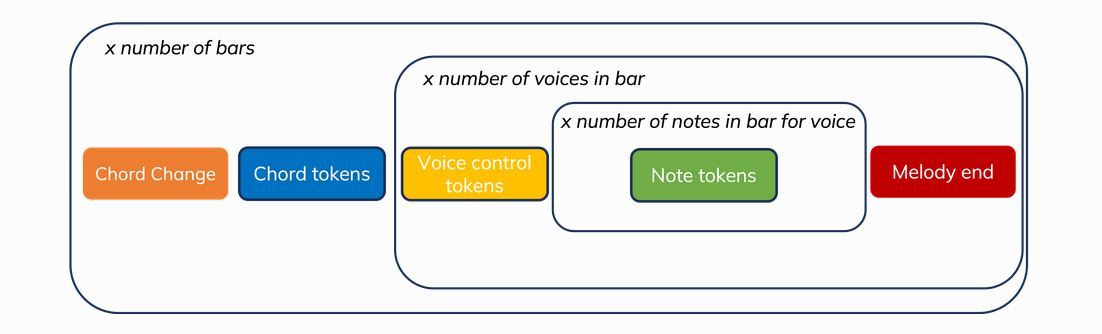
\includegraphics[width=1\textwidth]{IMAGES/MusicLang.JPG} 
    \caption{MusicLang's tokenization on a high level, shows a hierarchical tokenization process. At the highest level are chord-related tokens that describe the harmonic structure of a section. This is followed by instrument-level tokens that encode summarizing features such as instrumentation, octave, range, and note-density of a voice within a section. Finally, there are note-level tokens that encode the pitch and duration of an event within a voice within a section}
    \label{fig:musiclangtok}
\end{figure}

\subsection{RhythmLang}
RhythmLang is a fine-tuned variant of MusicLang with controls for inner metric weight. The fine-tuning targets the \textit{controlled continuation} and the \textit{controlled generation} modes of the model. Here the user provides a MIDI file as input from which inner metric weight is extracted and passed to the model. In \textit{controlled continuation} the user provides two MIDI files, one from which the model continues and one from which the model extracts the target metric weight profile. 
\section{Developing the Model}


\subsection{Preliminary Experiments - proof of concept}
The current methods of adding musical control to an existing model are poorly systematized and rarely compared to each other. While this thesis does not aim to provide a systemic comparison and experimental evaluation of different control methods, some preliminary experiments are necessary to establish a good course of action. We use BassCraft, a smaller model, and start by controlling for note density. Note density is more easily calculated, tokenized, and verified than inner metric weight. Once control for note density is established, we will move on to inner metric weight. \textbf{Addition} BassCraft is used as a proof of concept for the methods of adding control, it is not part of the final model and evaluation. The most promising approach, or combination of approaches will be applied to fine-tune MusicLang. 

\subsubsection{BassCraft -  a tiny transformer model}
To avoid wasting computing resources and energy, we perform the preliminary experiments on a smaller model: Basscraft. BassCraft is a small transformer model based on  GPT2 \cite{Radford_Wu_Child_Luan_gpt2_2019}. It has an embedding size of 256, 4 attention heads, four hidden transformer layers, and 7 million trainable parameters. In contrast, the target LLAMA 2-based model MusicLang has over 100 million trainable parameters. Basscraft generates a bassline to a provided piece of music and is trained on the Lakh MIDI dataset \cite{Raffel_2016}. For training, songs with bass lines are selected (based on the presence of particular MIDI-instrument channels). The tracks are divided into snippets between 1 and 16 bars long. The bass lines are separated from the remaining track and matched as potential output. 
\textbf{Addition} For inference, the user provides a target MIDI file $target$ and a MIDI bass instrument such as a Cello, or Electric Bass (see the appendix \ref{midi-bass}) for a full list of MIDI-bass instruments. The target MIDI file $target$ can be a single instrument or multi-instrumental track. The model generates a corresponding bass line of the same length as the target file (up to 16 bars). When we add control for note density, the user provides a single integer or a list of integers. If a single integer is passed, that integer is replicated across all generated bars. If a list of integers $X$ of size $|X|$ is provided, then the note density of bar $m$ is given by $X_{m\%|X|} \forall m \in target$
When control is added for inner metric weight, the user provides an additional reference MIDI file $reference$. The metric weight profile $W$ is given per bar $m$: $W_{m}$. The target rhythmic weight of a bar is given by $W_{m\%|W|} \forall m \in target$. The modulo operation ensures that for note-density and rhythmic weight control, the length of the control input does not have to match the length of the target midi file.    

\begin{figure}[H]
    \centering
    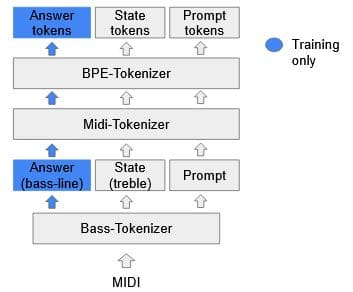
\includegraphics[width=0.5\textwidth]{IMAGES/Preprocessing1.jpg} 
    \caption{Preprocessing and tokenization of the original BassCraft model}
    \label{fig:preprocessing1}
\end{figure}

\subsubsection{Method 1 - Vocabulary Expansion}

Vocabulary expansion is the process of adding new vocabulary to a transformer model. MusicLang achieves its extraordinary controllability similarly to FIGARO \cite{Rütte_figaro_2023} using control tokens that summarize features of the music that go beyond simply representing MIDI-like events. In vocabulary extension, it is critical to ensure that additional tokens do not overwrite or collide with the existing training. Otherwise, the benefits of using a pre-trained model disappear. Since we use a BPE tokenizer, it is difficult to add new tokens, as it would require retraining the BPE tokenizer, which will transform the embedding layer, making the pre-trained model unusable. Instead, we investigate whether there are unused tokens and reassign them to our new control tokens. These new tokens are not included in any compound tokens generated by the BPE process, which increases the sequence length.

\begin{figure}[H]
    \centering
    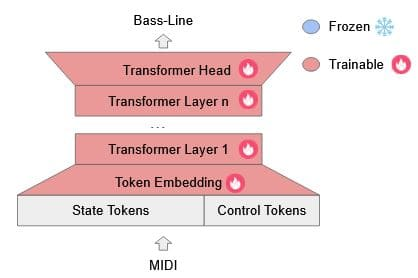
\includegraphics[width=0.5\textwidth]{IMAGES/full_ft.jpg}
    \caption{Vocabulary transfer with full fine tuning}
    \label{fig:vocabtrans1}
\end{figure}

\begin{figure}[H]
    \centering
    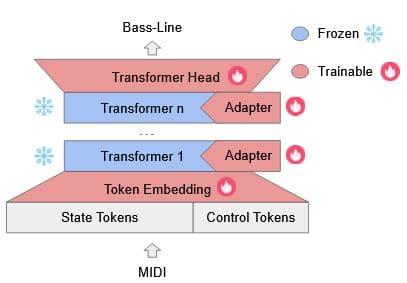
\includegraphics[width=0.5\textwidth]{IMAGES/vocab_lora_ft.jpg} 
    \caption{Vocabulary transfer with parameter efficient fine tuning}
    \label{fig:vocabtrans2}
\end{figure}

\subsubsection{Method 2 - Integrating of control tokens} 

This approach differs from vocabulary expansion because it processes the control tokens as a parallel stream. This is adapted from the approach used in Coco-Mulla \cite{Lin_cocomulla_2024}. After passing through a trainable positional embedding, the parallel stream of control tokens is inserted into the model at a layer $c$. The benefit of this method is that it doesn't require editing the model's vocabulary. 
 
\begin{figure}[H]
    \centering
    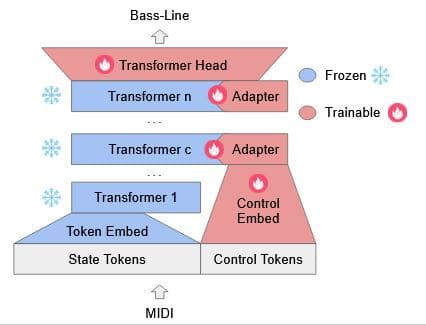
\includegraphics[width=0.5\textwidth]{IMAGES/ControlTokensLora.jpg} 
    \caption{Integration of control tokens with parameter efficient fine tuning}
    \label{fig:controltok}
\end{figure}

\subsubsection{Method 3 - Post-Hoc Guidance and other improvements}

SMITIN\cite{Koo_Wichern_Germain_SMITIN_2024} uses post-hoc guidance on a trained model to influence the generation process without retraining the model. This type of sampling-based guidance has been very successful in diffusion models. In transformers, however, it produces mixed results \cite{language_guide_rutte_2024}.  Additionally, this may be difficult to implement and transfer to IMA. Both SMITIN and Rütte\cite{language_guide_rutte_2024} only use one-dimensional variables that indicate the probability of a concept being present or not. 

\begin{figure}[H]
    \centering
    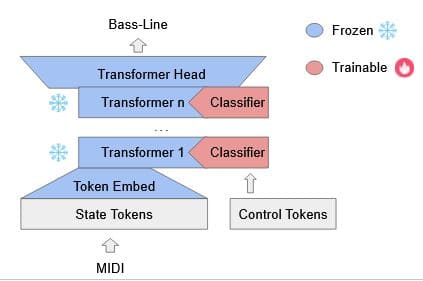
\includegraphics[width=0.5\textwidth]{IMAGES/adhoccontrol.jpg} 
    \caption{Integration of control using inference time interference}
    \label{fig:adhoccontrol}
\end{figure}

If these experiments are unsuccessful, we can follow the approach of \cite{Shu_Xu_Musebarcontrol_2024} and try additional training using auxiliary tasks or a modified (counterfactual) loss function. 

\subsection{Using inner metric weight as controllable feature}
Inner metric analysis (IMA) creates metric weight profiles we use as guiding features passed to the model bar by bar, which allows us to induce shifts in metric weight in the output. 
For this, we use the globally smallest available note grid of the Lakh MIDI dataset $g_min$. The calculated rhythmic profile is normalized and provided to the model as a vector of length $g_{min}$.
The model then learns embeddings of the distribution alongside positional embeddings \cite{Lin_cocomulla_2024}. These embeddings are incorporated into the model. For inference, the user can provide a reference track from which the inner metric profile is extracted and passed to the model. 

\subsection{Training RhythmLang}
Methods 1, 2, and 3 are sorted by expected difficulty of implementation. First, BassCraft is extended using each of the methods with control for note density. When a method is found that introduces sufficient control, we extend this to metric weight and try generating basslines with a provided metric profile. Finally, the most promising method (or combination of methods) is adopted to MusicLang, creating RhythmLang.

\section{Model Evaluation}
\subsection{Datasets}
\textbf{Addition} For fine-tuning the models with new control mechanisms, we use a small random subset of 1000 songs from the Lakh MIDI Dataset $lmd1000$. For BassCraft, we ensure that all songs in $lmd1000$ contain bass lines. Both BassCraft and RhythmLang are evaluated objectively using a second random subset of 500 songs from which a random subsection between 4 and 16 bars is selected for the \textit{continuation} mode of RhythmLang and the bass generation of BassCraft. This is the $lmd500$ evaluation dataset. The references for inner metric weight come from a small set of $n=30$ manually chosen prototypical rhythms $srhythm$ using the set by \cite{Chew_Volk_Lee_Dance_metric_weight_2005} of prototypical rhythms for Tango, Rumba BossaNova, Merengue, and March as a starting point. This can be expanded as desired for showcasing the control effectiveness.
To evaluate combined control of chords and rhythm we create a small set $n=30$ of different two, three, and four-bar chord progressions.
Finally, we create three datasets containing inferences from the model for evaluation, $bcraft\_inf$,  $mlang\_inf\_con$, $srhythm$. Each contains 500 entries, the model weights remain frozen during this process.  
To evaluate BassCraft we create $bcraft\_inf$ by running BassCraft on $lmd500$ with a randomly chosen rhythm from $srhythm$ as a control condition for each section in $lmd500$. 
To evaluate RhythmLangs's \textit{controlled generation} mode we create $mlang\_inf\_con$ by running RhythmLang on 500 different pairwise permutations of chords from $schord$ and rhythms from $srhythm$. 
To evaluate RhythmLang's \textit{controlled continuation} we run RhythmLang on $lmd500$ with randomly chosen rhythms from $srhythm$ for each track to create $mlang\_inf$, where RhythmLang continues from the excerpt from $lmd500$.  


\subsection{Evaluating Control-Effectivness}
As discussed in section \ref{section:evaluation}, calculating whether or not the control is effective depends on the controlled feature but can happen automatically. 
The first set of experiments targets note density: If note density is a categorical variable such as low, medium, or high, the error is calculated similarly to a multilabel classifier. The predicted label is the note density of the generated music, and the ground-truth label is the note density given in the prompt on a bar-by-bar level. 
The metrics include accuracy, precision, recall, and F1 scores. 
If note density is continuous (the number of notes per bar), then the error would be calculated as mean square error: 
\begin{equation}
 error_{continuous} = \sqrt{\frac{1}{n}\sum_{j=1}^{n}(y_{generated}-y_{prompt})}
\end{equation}
Inner metric weight analysis generates metric weight profiles, which we use as a guidance mechanism. Following the approach by \cite{Bemman2024}, we can compare the generated and the target rhythmic weight profiles using chi-squared distance.
Given target distribution $T$ and generated distribution $G$, the distance is given by 
\begin{equation}
D=\sum_{i=0}^{n-1}(\frac{(T_i-G_i)^2}{T_i+G_i})
\end{equation}
\subsubsection{}
To evaluate the success of inner metric weight control we compare the inference datasets 
\section{User Study}
\textbf{RQ2} and \textbf{RQ3} are evaluated through a user study. The goal is to recruit $n=20$ participants to complete a test of interactability and a survey comparatively evaluating the generated music. 
\subsection{Interactive Study}
The interactive study aims to evaluate the fitness of the controlled generated music from an MACT perspective. Specifically, in the MACT protocol used by Chalkiadakis \cite{Chalkiadakis_2022}, the patient is supposed to listen to changes in the music and change their playing. There are two options that we are deciding between.
\textbf{Option 1}
In our simplified interactive sessions, we ask the player to hit a button whenever they hear a change in the music. The button presses are registered alongside the starting time, tempo, and registered changing points (determined from the prompt). Finally, we correlate the timing of the button presses and registered changes are correlated with each other. A high correlation indicates that the participants noticed the changes. 
For this, we will generate $n=10$ long pieces using RhythmLang, with varying rhythm controls. As a control, we pass a MIDI file consisting of different template rhythms from $srhythm$ at random intervals concatenated into one file.   
\textbf{Option2}: We ask players to tap along to the music, and change their tapping when they notice a change. We analyze the regularity of the taps matching them with the music playing and investigate them for changes. 
For this, we will generate $n=10$ long pieces using RhythmLang, with varying rhythm controls. As a control, we pass a MIDI file consisting of different template rhythms from $srhythm$ at random intervals concatenated into one file.   

\textbf{Hypothetical hypotheses}: Players have more difficulty following generated music, generated with certain rhythmic templates than others. 
Players have more difficulty recognizing changes between certain rhythmic changes than others. 

\subsection{Survey}
The survey will compare the listening experience of our model to the rule-based music generation system used in the original game to answer RQ3, whether the music by RhythmLang improves listener experience.  The survey will also include the original MusicLang, to assess whether or not the fine-tuning for rhythm control decreases other capabilities of the model. Optionally, we include other symbolic music generators such as FIGARO \cite{Rütte_figaro_2023}, this will help provide a point of comparison. Following the recommendation of \cite{Yin_Reuben_Stepney_Collins_2023} we could also include a state-of-the-art rule-based generator such as MayaMarkov \cite{Collins_Laney_2017} and human-composed music from the Lakh MIDI dataset. 
The questionnaire will be adopted from \cite{Yin_Reuben_Stepney_Collins_2023}, and each musical excerpt will be rated on a 7-point Likert scale along the following dimensions: aesthetic pleasure, repetition, melody, harmony, and rhythm.\footnote{From \cite{Yin_Reuben_Stepney_Collins_2023}: Aesthetic pleasure (Ap) The extent to which someone finds beauty in something 
Repetition or self-reference (Re) The reuse, in exact or inexact form, of musical material (e.g., notes, melody, harmony, rhythm) within a piece.
Melody (Me) A succession of notes, varying in pitch, which have an organized and recognizable shape. Melody is horizontal, i.e. the notes are heard consecutively.
Harmony (Ha) The simultaneous sounding of two or more notes; synonymous with chords. The organization and arrangement of chords and their relationships
to one another, vertically (at the same time) and horizontally (across time) throughout a piece
Rhythm: Everything about the time aspect of music (as distinct from the aspect of pitch), including event or note beginnings and endings, beats, accents, measures, and groupings of various kinds.} 
Optionally there is space for the participant to comment on each excerpt. The participant will not see the source of the excerpt (i.e. which model, or whether or not it is generated). 
The music provided for comparison will be excerpts cropped to about 30 seconds of rendered MIDI. While we don't cherry-pick the tracks, we will follow \cite{Yin_Reuben_Stepney_Collins_2023} and filter the music to prevent 1) excessive repetition of a small sequence (the model getting "stuck"), 2) long stretches of silence, 3) verbatim copying of training data or the prompt. 
The questionnaire also includes questions on demographic information such as gender, age, educational background, and musical experience.

\textbf{Hypothetical hypotheses}: Ratings of aesthetic pleasure are higher for RhythmLang than for Chaldiakis's rule-based system. \\
Ratings of aesthetic pleasure are not higher for MusicLang than for RhythmLang. \\
Ratings of repetition, melody, harmony, and rhythm are positively correlated with ratings for aesthetic pleasure.\\
Ratings of rhythmic success are higher in RhythmLang with certain rhythm conditions than others. 

\subsection{Additional points of discussion}
For each of the musical dimensions aesthetic pleasure, repetition, melody, harmony, and rhythm, the difference in responses between the models is evaluated and significant differences $\alpha = 0.05$ are highlighted. 
Beyond simple statistical evaluation, I would include listening examples and an interactive code space on Google Collab where the reader can experiment with RhythmLang. Additionally, discussing participants' comments, and investigating the model output musicologically, could be worthwhile depending on the results. 
\section{Thesis Timeline}

\begin{figure}[H]
    \centering
    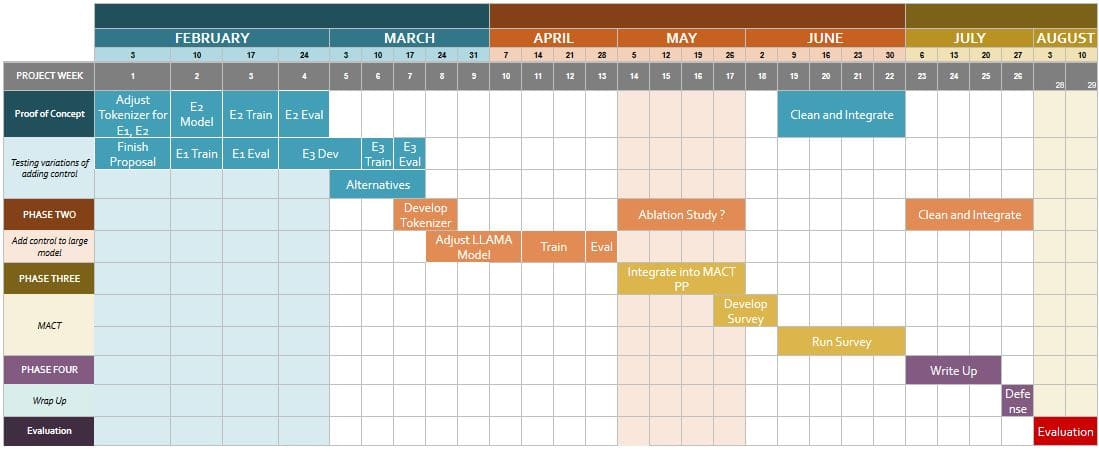
\includegraphics[width=1\textwidth]{IMAGES/project_plan.jpg} 
    \caption{Thesis project plan}
    \label{fig:projectplan}
\end{figure}


